\chapter{Methods} \label{chapMethod}
\section{Datasets}
In this work, we use data from a variety of sources. The first is from small, consumer-grade drones that capture only GPS-tagged images. This type of data is relatively easy to collect and representative of what is commonly available to foresters today. The second type of data is from a custom drone payload that records data from multiple sensors at once. This type of rich data has only been collected in limited research settings in forestry. An overview of these datasets can be found in Table \ref{table:methods:drone_datasets}. The third type of data is existing data from remote sensing, specifically an aerial mapping survey that is freely available. Finally, we use annotated forestry data that was captured from a ground vehicle perspective and procedurally generated synthetic data from the same environment. We use this as training data for our system. These datasets are summarized in Table \ref{table:methods:non_drone_datasets}.

\subsection{Commodity Drone Data}
We use data collected with a DJI Air 2s, a small commodity drone that is commonly used for videography. The data was captured in Stowe, Vermont in the Northeastern United States. The drone was flown in a lawnmower survey pattern at an altitude of 100 meters and the camera was oriented in the downward facing, \textit{nadir}, perspective. This data consists of 225 un-calibrated images that are geo-tagged with commodity-grade GPS measurements.

\subsection{Multi-Sensor Drone Data}
Many modern approaches to simultaneous localization (SLAM) and semantic mapping require as input multiple sensing modalities, such as cameras, LiDAR, IMU, and GPS. Therefore, other members of our team built a multi-sensor payload that could be mounted on a drone, as seen in Figure \ref{fig:methods:payload}. 
This payload is modular and could be mounted to different drones with different inclination angles. In these experiments, we used two large commercially-oriented drones, a DJI Matrice 600 and an AltaX Freefly. We flew a variety of different experiments, both under the canopy and over the canopy. In the under-canopy settings, we flew in small clearings between trees in Portuguese forests under manual control. Babak B. Chehreh, an experienced drone pilot from the University of Coimbra, controlled the drone during these data collections. In these experiments, we surveyed the boundary of the clearing exhaustively by using an oblique payload orientation of 30 degrees from horizontal. This technique was used to collect the \textit{Oporto} and \textit{Coimbra} datasets.

\begin{figure}
    \centering
    \includegraphics[width=0.55\textwidth]{figs/methods/datasets/payload_annotated.pdf}
    \hfill
    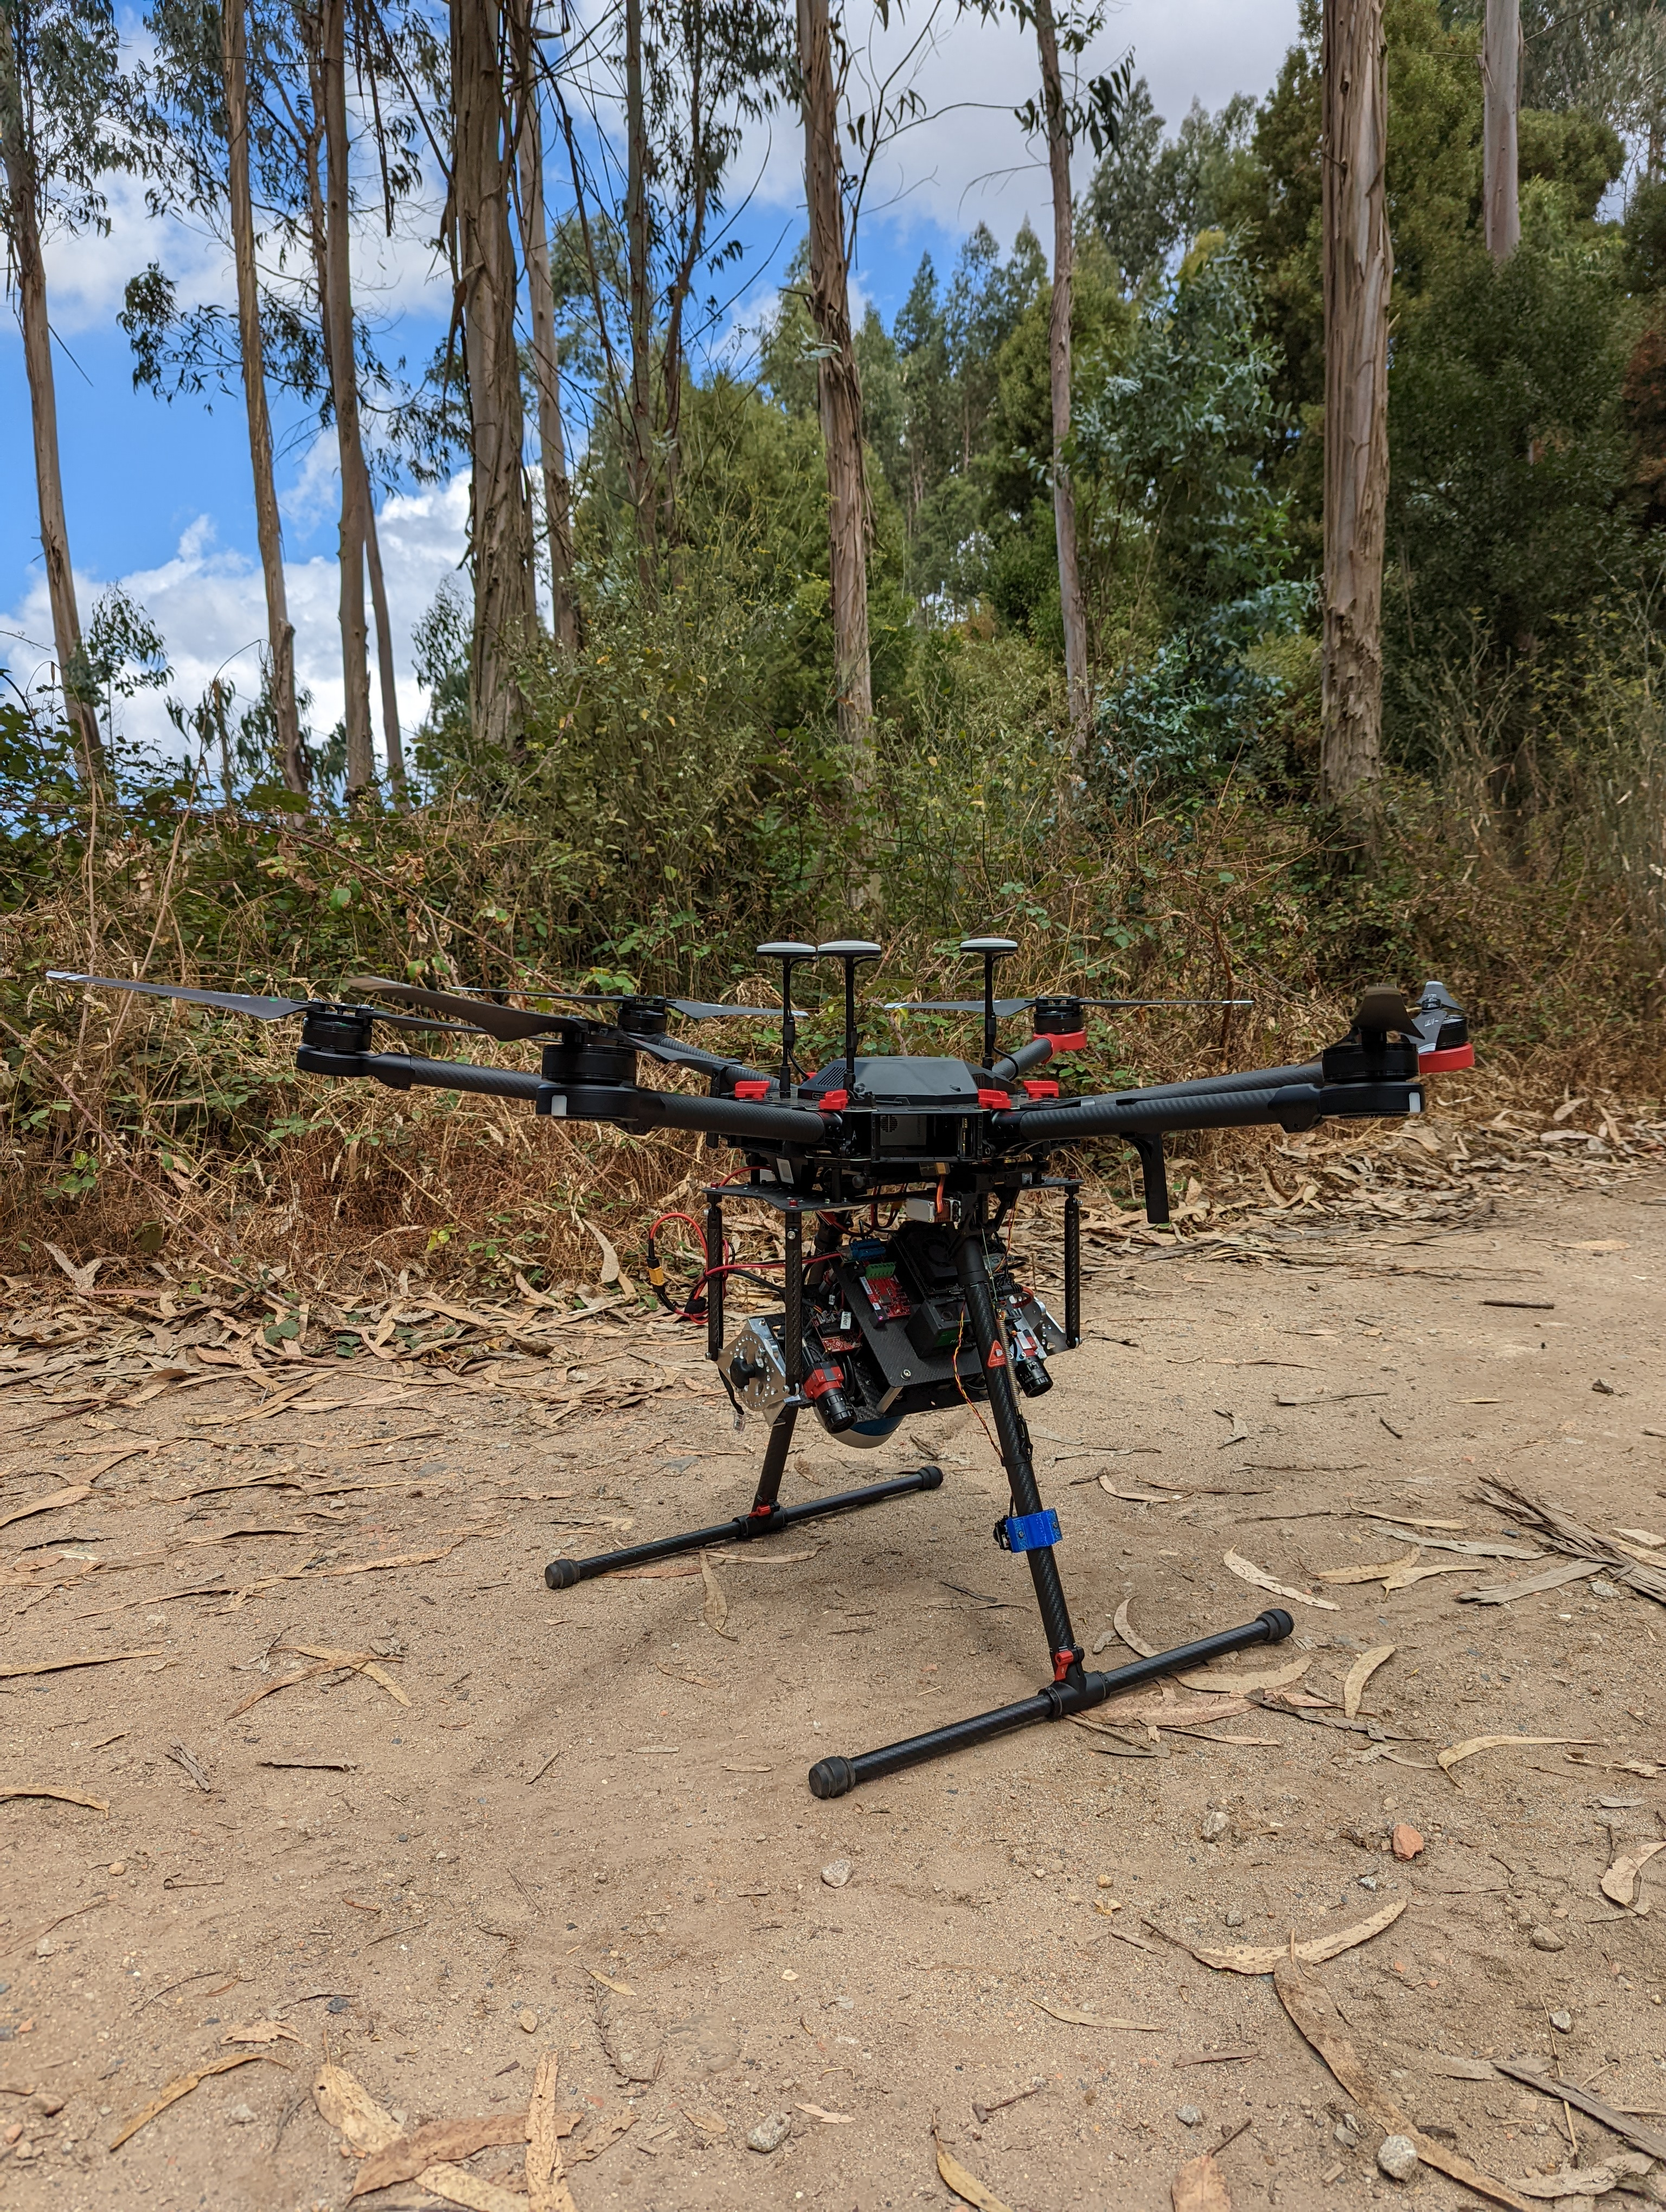
\includegraphics[width=0.37\textwidth, clip=true, trim={0cm 16cm 0cm 40cm}]{figs/methods/datasets/payload_on_drone_portugal_3.jpg}
    \caption{On the left is the multi-sensor payload developed by other members of our team. It consists of a LiDAR, stereo RGB camera pair, a multispectral camera, an IMU and a GPS. It also has onboard computation and storage. In most experiments, we used this platform onboard a DJI Matrice 600, pictured right. Photo credits to Winnie Kuang.}
    \label{fig:methods:payload}
\end{figure}


We also conducted a more conventional over-canopy survey using an automated flight planner. We executed a lawnmower coverage pattern over a test site in Pittsburgh, Pennsylvania USA that consisted of trees, shrubs, grasses, and bare earth. This was conducted at an altitude of 40 meters with the payload facing forward at a slight off-nadir angle of 75 degrees from horizontal. This data is labeled \textit{Gascola} after the name of the area we tested in.

The primary value of this platform was to collect rich multi-sensor data. It also allowed us to roughly replicate the type of data that would have been have been obtained from a commodity drone, such as that described in the previous section. This was done by taking images from a single camera and geo-tagging them with the drone's GPS. We conducted one study where the drone was flown manually in an orbital pattern with an off-nadir payload inclination, so the payload faced outward. This data was collected in the Wharton State Forest in New Jersey, USA, over a coastal pine barren, and is called \textit{Wharton}. Due to a sensor malfunction, this data does not have GPS information.



\begin{table}[]
\centering
\begin{tabular}{|l|l|l|l|l|}
\hline
\textbf{Name} & \textbf{Location} & \textbf{Platform} & \textbf{Environment} & \textbf{\makecell{Flight Pattern\\(camera degrees \\from horizontal)}}\\
\hline
Stowe & \makecell{Stowe,\\ VT USA} & \makecell{DJI Air 2s} & \makecell{Forest} & \makecell{Lawnmower (90)} \\ 
\hline
Coimbra & \makecell{Coimbra,\\ Portugal} & \makecell{Multi-sensor \\ payload \\(camera only)} & \makecell{Forest path} & \makecell{Manual out \\and back (30)} \\ 
\hline
Wharton & \makecell{Hammonton,\\ NJ USA} & \makecell{Multi-sensor \\ payload \\(camera only)}  & \makecell{Forest with road} & \makecell{Manual oval \\ over canopy\\ (60)} \\
\hline
Oporto & \makecell{Oporto,\\ Portugal} & \makecell{Multi-sensor \\payload} & \makecell{Forest clearing\\ with grass} & \makecell{Manual observations\\ of the boundary (30)}\\
\hline
Gascola & \makecell{Pittsburgh,\\ PA USA} & \makecell{Multi-sensor \\ payload}  & \makecell{Trees, shrubs,\\ and grasses} & \makecell{Lawnmower \\ over canopy\\ (75)} \\
\hline
%Emerald \cite{Young2022} & \makecell{Lake Tahoe,\\ CA USA} & \makecell{DJI Mavic 2} & \makecell{Forest} & \makecell{Lawnmower (90)} \\ 
%\hline
\end{tabular}
\caption{A summary of drone datasets used in this work.}
\label{table:methods:drone_datasets}
\end{table}

\subsection{Forestry Data from the Ground Perspective}
Because there is a lack of public annotated forestry datasets from the drone perspective, we used two existing datasets from a ground vehicle perspective. The first consisted of 121 multispectral images of a Portuguese forest collected by Andrada et. al. \cite{Andrada2020}. These images were manually segmented by the authors into six classes: background, live flammable material (aka fuel), canopies, trunks, humans, and animals. The original paper uses multi-spectral data but we only used the co-registered RGB data that was released. This choice allowed us to deploy the model on the RGB camera onboard our payload, rather than trying to integrate a multispectral camera with similar spectral properties. We refer to this dataset as \textit{Sete Fontes} because it was collected in a region with that name.

We also used a synthetic dataset rendered from a procedurally-generated Portuguese forest as described by Nunes et al. \cite{nunes2021procedural}. In this work, the authors procedurally created a forested landscape by first creating the terrain, then placing paths and rocks, and finally adding vegetation. After generating the terrain, they rendered photorealistic images using computer graphics techniques. These renders were created at regular intervals along a simulated ground vehicle trajectory, resulting in 3154 images. They also rendered another image using the same mesh and camera position that described what type of object was observed at each pixel. These classes were slightly more-granular than those used by Andrada et al. \cite{Andrada2020}, but they could easily be aggregated to match the former. There were no examples of humans or animals in this simulated dataset, but these classes were not critical to this work and only occurred infrequently in the \textit{Sete Fontes} dataset. 

\subsection{Optical Remote Sensing Data}
In this work, we focus primarily on data collected by the National Aerial Imagery Program (NAIP) multi-spectral data source which contains red, blue, green, and near-infrared bands. This data is collected at an interval of at most every three years over the continental US. The USDA contracts with states to obtain this data from manned aerial surveys. The data is post-processed to provide an ortho-rectified, stitched, and geo-referenced product analogous to satellite imagery. The resolution per pixel is 0.6 meters, which is the highest-resolution freely available multispectral data we are aware of for the US. An example image can be seen in Figure \ref{fig:methods:NAIP_example}. The quality of this data has recently been largely superseded by commercial satellites such as Planet Labs \cite{Planet}, but this data is not freely available and therefore not as useful for research purposes. 

\begin{figure}
    \centering
    \includegraphics[width=0.5\textwidth]{figs/methods/datasets/NAIP_example.png}
    \caption{An example NAIP image crop at a resolution of 0.6 meters per pixel. Land cover classes are generally easy to interpret, but small details are lost.}
    \label{fig:methods:NAIP_example}
\end{figure}

\begin{table}[]
\centering
\begin{tabular}{|l|l|l|l|l|}
\hline
\textbf{Name} & \textbf{Location} & \textbf{Type} & \textbf{Environment} \\
\hline
Sete Fontes \cite{Andrada2020} & \makecell{Coimbra,\\ Portugal} & \makecell{Under-canopy \\ images} & \makecell{Forest} \\ 
\hline
Synthetic \cite{nunes2021procedural} & \makecell{Simulation of \\ Portugal} & \makecell{Under-canopy \\ images} & \makecell{Forest} \\ 
\hline
NAIP \cite{U.S.DepartmentofAgriculture2011NationalSheet} & \makecell{Continental US} & \makecell{Aerial imagery} & \makecell{Varied} \\ 
\hline
 Chesapeake LULC \cite{Claggett2014ChesapeakeProduction, Robinson2019LargeData} & \makecell{Chesapeake Bay,\\ US} & \makecell{Annotated \\ Land Use/\\Land Cover\\ segmentation} & \makecell{Varied} \\ 
\hline
\end{tabular}
\caption{Summary of non-drone datasets used in this work}
\label{table:methods:non_drone_datasets}
\end{table}

%\subsection{Data management}
%A practical consideration when dealing with this much data is how to effectively store, version, organize, and share it in a seamless fashion, especially when working in collaborative teams. The tool used for managing the complexities of software development, such as `git`, have similar goals but do not support managing large, non-text files. 
%Cloud hosting and local harddrives inenvitably become challenging to organize and do not natively support a versioning system, which makes them susceptible to accidental errors or duplicated data. 
%In this work, we leveraged a software tool called Data Version Control (DVC), which is designed for organizing data in large projects such as machine learning and data science. DVC acts as a management layer between a git-tracked project and an arbitrary remote storage device. Effectively, DVC creates light plaintext files which describe the real data. These a small files can be tracked by `git` and represent a full history of the project.  
%
%We created a `git` repo and associated `DVC` datastore for each project we worked on that had a different goal. Our organizational strategy evolved over time, but at the end involved two main concepts: a standardized hierarchy to organize the different data collects and a level designation to sort data based on the level of processing. The organizational structure was as follows `site\_name -> YYYY\_MM\_DD -> collect\_NNN` A site name represented one location where we collected data. This was chosen as the top-level organizational structure because data from the same site is most commonly used together. The next level represented the date and the final level broke the data up into logical segments. In general this corresponded to one drone flight, but in rare instances represented multiple flights where we left the sensors logging continuously, or data collected solely on the ground for calibration purposes. The level designation was inspired by the satellite community, where different levels denote different steps of sequential post-processing. In our work, we used Level0 to represent raw data, as copied from the platform. Level1 represented data processed into a standarized format. This was less important for commodity drone data, since it was frquently already captured as folders of geotagged images. However, it was very important for extracting easy-to-use information from rosbags, which is how our multi-sensor custom data was stored. Level2 represnted processed results such as structure from motion and semantic predictions. In initial work, we nested all the levels within a collect. However, we later found that for our usecases it was easier to have levels be the top level organizational structure. This allowed us to quickly check for all datasets matching a specific level of processing. The final organaiztional structure was as follows:
%
%% TODO fix this up
%
%\begin{verbatim}
%    
%├── level_00
%│   ├── README.md
%│   ├── <site_name_x> # A different folder for each geographic location
%│   │   └── <date_YYYY_MM_DD> # A different folder for each day at that site
%│   |       ├── collect_<NNN> # A different folder for each collect, which is probably synonmous with a flight
%│   │       └── collect_<NNN>
%│   └── <site_name_y>
%│       └── 2023_06_15
%│           ├── collect_<NNN>
%│           └── collect_<NNN>
%├── level_01 
%│   ├── README.md
%│   └── per_collect # Data in easy-to-use format, structured like level_00
%│       └── README.md
%└── level_02
%    ├── README.md
%    └── photogrametry # Photogramtery results
%        ├── README.md
%        └── metashape # Could have multiple softwares
%            └── per_collect # Structured like level_00
%\end{verbatim}

\section{Geometric Understanding of Forests using Drone Data}


\subsection{Photogrammetry}
\label{sec:methods:photogrammetry}
We conducted photogrammetry experiments using a variety of datasets. These were collected by both the commodity drone and the custom payload. For the commodity drone, we used all of the data that was collected and did not have to apply any post-processing. This is because the images were only collected after the drone had moved a sufficient distance to avoid redundancy. Additionally, the GPS location where the image was captured was embedded in the metadata.

The data from our custom payload required post-processing to prepare it for the structure from motion software. These images were captured at a high frequency of 10 HZ so consecutive images were often highly redundant. As shown by Young et al. \cite{Young2022}, highly redundant images contribute little to the overall quality but we found them to dramatically increase computation times. Therefore, for custom drone payload, we down-sampled the image to 2HZ. If we had GPS data available for the dataset, we tagged each image with the GPS coordinate from the temporally-nearest GPS record.   

We found in preliminary experiments that Agisoft Metashape \cite{AgisoftMetashape}, a commercial structure from motion software, consistently produced high-quality results. This software was also used in the work of used by Young et al. \cite{Young2022} for creating models from drone images of conifer forests in the Western US. This work recommends parameters image alignment and depth map creation, which are the first two steps in the Metashape pipeline. We use these recommended parameters in our experiments. Their work does not provide a recommendation for the later mesh generation and orthomosaic computation steps, so we use the default Metashape parameters which largely prioritize quality over computational time. 

\subsection{Simultanous Localization and Mapping}    
Since SLAM is not the focus of this work, we choose to use results from our collaborators on these datasets. We use two methods from their experiments, LIO-SAM \cite{Shan2020LIO-SAM:Mapping} with the parameters tuned for the forestry domain and a custom SLAM algorithm that combines components of both LIO-SAM and VIL-SLAM \cite{Shao2019StereoMapping} to use information from both LiDAR and stereo vision in a tightly-coupled manner. A thorough description of this system can be found in \cite{RussellUnmannedMitigation}. Both of these approaches provide a continuous estimate of the drone's position and orientation with respect to a static world frame.

\section{Tree Detection in Top-Down Data}
\label{sec:methods:tree_det}
The goal of this work is to study tree detection using multiple types of input data. We consider three sources: aerial imagery, drone imagery, and manual surveys that can provide the location and size of a small patch of trees. The first question we aim to address is the comparative accuracy of tree detections from drone versus aerial imagery using DeepForest \cite{Weinstein2020DeepForest:Delineation}. The second is the utility of different site-specific fine-tuning methods compared to simply using the default DeepForest model that is trained on diverse data from the NEON sites across the US. Our goal is to determine whether aerial data such as NAIP is sufficient for detecting trees or whether additional effort must be put in to collect drone imagery and/or field measurements. 

For these experiments, we assume that the ground truth trees are fully within the region the drone surveyed and the drone survey be fully within the region covered by satellite data. This is a realistic model for a situation where a forester measured the trees in a region and then flies a drone to survey the surrounding area. The remote sensing data could be taken from any relevant available source, such as NAIP. An example of the scale of the different types of data can be seen in Figure~\ref{fig:methods:multi_scale_tree_det}.

\begin{figure}
    \centering
    \includegraphics[width=0.3\textwidth]{figs/methods/tree_detection/multiscale_outset.png}
    \includegraphics[width=0.3\textwidth]{figs/methods/tree_detection/multiscale_inset.png}
    \includegraphics[width=0.3\textwidth]{figs/methods/tree_detection/multiscale_in_inset.png}
    \caption{The experimental setup with broad-coverage aerial data, medium coverage drone data, and a small set of ground truth tree locations. The same data is visualized at three different scales for clarity.}
    \label{fig:methods:multi_scale_tree_det}
\end{figure}

\begin{figure}
    \centering
    \includegraphics[width=0.45\textwidth]{figs/methods/tree_detection/annotations/stow_anew_2023_06_15_collect_000_manual_000_ortho_mesh_georef_train_annotations_2.png}
    \includegraphics[width=0.45\textwidth]{figs/methods/tree_detection/annotations/naip_crop_m_4407237_nw_18_060_20210920_train_annotations_5.png}
    \caption{Training data from the drone orthomosaic (left) and NAIP (right).}
    \label{fig:methods:tree_det_data}
\end{figure}


The first step in this experiment was processing the drone images into an orthomosaic, as described in Section \ref{sec:methods:photogrammetry}. This orthomosaic had a resolution of approximately 3 centimeters per pixel. Since the drone has GPS, this orthomosaic is roughly registered to a global reference frame. However, there are some errors in the GPS measurements and we noticed a slight mis-registration in both scale and translation. We precisely aligned the orthomosaic to our aerial data using QGis \cite{QGIS_software}. This provides an interface to select corresponding points between the two datasets. Then, QGis optimizes a translation and scale transform to best align the orthomosaic to the aerial data. 

The overall goal of this work was to assess the performance of a deep learning method for tree detection. We chose to use DeepForest \cite{Weinstein2020DeepForest:Delineation} because it is widely used and trained on a comprehensive dataset.
The authors state that spatial resolution and the size of the sliding window crop are especially important to the performance of DeepForest on new data. In preliminary experiments, we re-sampled the orthomosaic from the drone data to a variety of resolutions. We applied the pre-trained DeepForest model and qualitatively assessed the quality of the predictions at the different resolutions. We found that the best performance was at 0.1 meters per pixel, which was the same resolution the model was trained on. Therefore we re-sampled both datasets to this resolution. This resulted in down-sampling (coarsening) the drone data and up-sampling (interpolating) the aerial data. We used the default window size of 400 pixels, which was also the size used for training. An example of the training data can be seen in Figure \ref{fig:methods:tree_det_data}.

DeepForest was trained using the default setting of the Adam \cite{} optimizer. The model was trained for 200 epochs on the manual annotations and scaled down by the number of annotations for the drone predictions, to train for X epochs. For the pretrained model, release X was used.


\section{Semantic Mapping of Forests}
\label{sec:methods:sem_mapping}
The goal of our semantic mapping experiments was to determine the location of forest fire fuel within the environment. Unfortunately, the definition of what is fuel is often vague, such as "anything that can burn is fuel for a fire," according to the US Office of Wildland Fire \cite{Fire2021FuelsManagement}. Therefore, in our work, we focused on segmenting the environment into four broad classes, canopy, trunks, bare earth, and ground vegetation. Since the goal was to inform an automated ground vehicle, we labeled ground vegetation class \textit{fuel}.

Semantic mapping can be done with a variety of sensing modalities. A relevant work on semantic mapping for forestry, SLOAM \cite{Chen2020SLOAM:Inventory}, focuses solely on detecting tree trunks within the environment and building a 3D map where trunks are represented as cylinders. Because of the distinctive geometry of trunks, they are able to detect them in LiDAR scans. Since we want to distinguish classes that may have similar local geometry, we cannot base our predictions on LiDAR and instead choose to predict semantics using images, as done in the work of Andrada et. al. \cite{Andrada2020} in the ground vehicle setting. Using images has the added benefit that it is relatively easy for humans to label annotated data for training. This is in contrast to labeling LiDAR data, which takes significant effort as described in SLOAM. Moreover, there are a wide range of semantic segmentation models available that are conceptually interchangeable. 

\subsection{Semantic Segmentation} \label{sec:semseg}
To the best of our knowledge, there are no publically available pre-trained models that are useful for our task of vegetation classification in forests using RGB data. Therefore, we needed to train our own models. We conducted two experiments, one on the \textit{Oporto} dataset from Portugal and another on the \textit{Gascola} dataset from the US. 

In the Gascola experiments, our objective was to segment the different classes from overhead imagery. Since there weren't any relevant datasets, we chose to label a small amount of data on our own for training. When creating semantic segmentation training data, it is very time-consuming to label the boundaries between each class precisely. This is especially true for natural environments, where different classes are often interlaced at the boundary, such as tree branches over the ground or bare earth transitioning to grass. A relevant work on segmenting ground cover with drones is Davila et. al. \cite{Davila2022ADAPT:AI}, where they showed that coarsely labeling regions away from class boundaries was much faster, and the model trained on these coarse annotations still made accurate predictions at the boundaries.

We conducted manual annotations using the VIAME toolkit \cite{Dawkins2017AnAnalytics}, a free and open-source web annotator. Even though our primary goal was to only distinguish broad classes, we chose to annotate a more granular set of classes loosely inspired by the Anderson13 fuel model \cite{anderson1981aids}, a vegetation classification system commonly used in fire modeling. These granular classes, along with their mapping to aggregated classes, can be seen in Table \ref{table:methods:fuel_classes}. Our reasoning for labeling fine-grained classes was that this allowed us more flexibility when it came to future experiments, where we might want to aggregate the classes differently. Furthermore, it gave us the option to train on these classes and aggregate them after prediction. In practice, we found that this additional granularity did not increase the labeling burden significantly, since we rarely had to break up spatial regions that would have originally been considered one coarse class. Rather, we mostly labeled entire regions with more granular designations. 


%\begin{figure}[!ht]
%    \centering
%    \includegraphics[width=\linewidth]{figs/methods/semantic_mapping/viame_example.png}
%    \caption{Example manual annotations using the VIAME toolkit, a free and open source web annotator with potential support for integrated model training.}
%    \label{fig:methods:manual-annotations}
%\end{figure}

\begin{table}[ht!]
    \centering
\begin{tabular}{ccc}
% \hline
\toprule
\textbf{Fine-grained class} & \textbf{Coarse-grained classes} \\ \midrule
Dry Grass          &  Fuel \\
Green Grass        &  Fuel \\
Dry Shrubs         &  Fuel \\
Wood Pieces        &  Fuel \\
Litterfall         &  Fuel \\
Timber Litter      &  Fuel \\
Green Shrubs       &  Canopy \\
Canopy             &  Canopy \\
Live Trunks        &  Canopy \\
Bare Earth         &  Background \\
People             &  Background \\
Sky                &  Background \\
Blurry             &  Background \\
Drone              &  Background \\
Obstacle           &  Background \\
% \hline
\bottomrule
% \hline
\end{tabular}
\caption{Classes used in semantic segmentation. These are inspired by relevant classes from the Anderson13 fuel model \cite{anderson1981aids} and also include additional classes relevant to our application.}
\label{table:methods:fuel_classes}
\end{table}

We use a segmentation network based on a transformer architecture called SegFormer \cite{Xie2021}. Given the relatively low amount of real-world images in our training dataset, this network was especially suitable since it showed strong performance on benchmark datasets and good generalization capabilities. We trained this model using the default parameters used in the MMSegmentation \cite{mmseg2020} implementation. 


\subsection{Semantic Mapping with a Camera and LiDAR}

\begin{figure}[!ht]
    \centering
    \includegraphics[width=\textwidth, clip, trim={0 1.5cm 0 1.8cm}]{figs/methods/semantic_mapping/semantic_mapping_overview.pdf}
    \caption{An overview of the LiDAR-camera semantic mapping system}
    \label{fig:methods:lidar-camera-semantic-mapping}
\end{figure}

We modified an approach for RGB-D semantic mapping \cite{semantic_slam} to use LiDAR instead of per-pixel depth data to perform geometric reasoning. First, each RGB image is passed through the best semantic segmentation network from Section \ref{sec:semseg} to get a classification result for each pixel. Using the extrinsic parameters relating the LiDAR's orientation and position to the camera, we transformed the LiDAR measurements into the camera's coordinate frame. Then, using the calibrated camera intrinsic, we project each LiDAR point into the image plane. Points within the field of view of the camera are assigned a classification label from the corresponding pixel in the semantic map. This semantically-textured point cloud is transformed into the inertial reference frame using the current pose of the drone estimated by our SLAM system. 

We use an octomap \cite{hornung13auro} representation to efficiently discretize the generated semantic point cloud into voxels. Each voxel has a resolution of 0.05m and contains information about the predicted classification. Each time a new semantic point cloud is created, it is used to update the global octomap. Since each voxel can contain multiple observations, we use two approaches to determine the aggregate classification. The first method assigns the class label using the highest-confidence prediction from the neural network that corresponds to that voxel. Alternatively, we use a Bayesian method which maintains a probability distribution over the classes. Each new observation is multiplied by the current distribution and then re-normalized. The voxel is then labeled with the most probable class. An overview of the proposed system can be seen in Figure \ref{fig:methods:lidar-camera-semantic-mapping}.


\section{Informative Path Planning}
Automated methods for interpreting remote sensing data are often developed using a sparse set of accurate field measurements. An example of this is the LANDFIRE project, which uses user-submitted plot data about vegetation type to build a prediction model for LandSat data \cite{LANDFIRE2018ValueLANDFIRE}. Drones have the potential to automatically classify vegetation types as described in Section \ref{sec:methods:sem_mapping} and these drone predictions, if accurate enough, could be used to inform the satellite model. 
A natural question is where to collect sparse drone observations so that they effectively model the surrounding region. 
Intuitively, the samples should be diverse and focus on examples that are expected to be the most interesting class or most challenging to classify. This intuition is challenging to implement in a domain-flexible way while also respecting operational considerations.
A major constraint is that drones have a finite battery life which governs the distance they can cover before returning home to have their battery replaced. This means that the distance of any one flight is bounded. Commodity drones do not expose the ability to algorithmically control the drone in real-time based on the sensor inputs, so the entire trajectory must be planned before the drone takes off.
We make some simplifying assumptions to define the type of observations we take. Specifically, we assume that the atomic observation is a plot or a small lawnmower survey of a fixed square size. We further assume that the user specifies a fixed number of plots to visit. Since it will take a fixed amount of time to execute the plot surveys, the maximum available time to traverse between plots is the maximum time of a full flight minus the time taken to complete the surveys. The algorithm's decision variables are where to place these plots and in what order to visit them, subject to the maximum time available to traverse between them.


A good choice of plots depends heavily on the task that is being conducted. However, it's possible that the data may be used for multiple purposes or the method of conducting the task has not been defined when the data is collected. To make our system as general as possible, we assume that in the absence of any other information, collecting a diverse and representative set of samples is desirable. To implement this concept, we need some notion of similarity that is applicable to a variety of domains and input data. We also need a planner that uses this description of diversity to plan a set of observation plots that are diverse and representative.


%\subsection{Feature Extraction on Remote Sensing Data}
%\begin{figure}
%    \centering
%    \includegraphics[width=0.5\textwidth]{figs/methods/IPP/TSNE_features.png}
%    \caption{Unsupervised features separate classes in a t-SNE embedding.}
%    \label{fig:methods:tsne_feature_embedding}
%\end{figure}

Feature extraction is the process of converting raw data into a format that captures attributes that might be useful for machine learning. In classical computer vision, feature extraction or ``feature engineering" was a widely-studied topic. Many works attribute the success of deep learning to the informative features that are extracted in the early layers of the network. These are optimized for the target problem through the neural network training process. Since it takes a large amount of labeled data to train these features, it is common to use the first layers of a network trained for one task as a feature extractor or ``backbone" for another related task that has less labeled data. However, applicable pre-trained models are not yet ubiquitous for remote sensing, especially given the diversity of modalities. Multiple approaches have been proposed to extract unsupervised features using paired modalities \cite{Xie2016TransferMapping} spatial correlations \cite{Jean2019Tile2Vec:Data} or layer-wise greedy training \cite{Romero2016UnsupervisedClassification}. In all cases, this still requires training a new network as a feature extractor which can be technologically difficult and computationally intensive.

A recent work called MOSAIKS \cite{Rolf2021} proposes random convolutional kernels as a strong alternative to pre-trained deep networks for feature extraction. Specifically, they suggest using small crops, e.g. 3x3, from the dataset as convolutional filters and then applying a non-linear activation. This process is extremely computationally efficient and notably requires no neural network pre-training. The authors show that these features are remarkably good for a variety of predictions on geospatial data. Specifically, they are better than using a CNN pre-trained on a different task as a feature extractor, and almost as good as a CNN trained for the task in question.

Because of the strength and flexibility of this approach, we use it as the basis for our feature extraction method. The original work uses 1024 kernels to extract features, so the features consist of significantly more data than the input. This is because the convolutional features are produced at the same resolution as the input image. In their work, the authors address this issue by spatially averaging the data across large cells. However, in our work, we require features that capture variation on a local level. Therefore, we retain the spatial resolution but reduce the number of features with dimensionality reduction. This technique was employed in a related informative path planning work by Candela et al. \cite{Candela2020PlanetaryMapping}, except the input was hyperspectral data rather than the convolutional feature maps. In both cases, the features are highly correlated with each other, so much of the information can be represented by a significantly smaller number of features. We use Principal Component Analysis (PCA) \cite{Jollife2016PrincipalDevelopments}, a widely used statistical technique for reducing the dimensionality by finding the linear projection that retains the most variance in the original data. We use the first 6 principal components as features. This number of features was chosen because preliminary classification experiments showed performance plateaued after this number. A useful property of PCA is that the features it produces are uncorrelated. To make our feature representation even more consistent, we standardize each feature to have zero mean and unit variance. An example of feature extraction can be seen in Figure \ref{fig:methods:unsupervised_features}. This shows that different types of land cover have different feature representations.

\begin{figure}
    \centering
    \includegraphics[width=0.3\textwidth]{figs/methods/IPP/img_for_features.png}
    \includegraphics[width=0.3\textwidth]{figs/methods/IPP/first_three_feaures.png}
    \includegraphics[width=0.3\textwidth]{figs/methods/IPP/second_three_features.png}
    \caption{Example unsupervised features generated by MOSAIKS and PCA. The first image is the input data and the next two images are the six features, visualized as the channels of two RGB images. For visualization, the data is centered at 0.5 and clipped at the third standard deviation.}
    \label{fig:methods:unsupervised_features}
\end{figure}

\subsection{Gaussian Process Uncertainty Modeling}
The goal of extracting meaningful features is to enable uncertainty modeling.
Gaussian Processes (GPs) \cite{Rasmussen2004} are a principled tool for quantifying prediction uncertainty. They are a kernel-based method, where the kernel defines the similarity between two features. This can be fit to data or set using expert knowledge. Because of this, they are used as a key component of works on sensor placement \cite{Krause2008Near-optimalStudies} informative path planning \cite{Fernandez2022InformativeAnalysis, Candela2020PlanetaryMapping, Candela2021}. An important property of GPs uncertainty is that it only depends on the features and not the associated values. This makes them applicable to offline planning. In contrast, uncertainty estimation approaches built on ensambles of prediction models require the label of a proposed sample to compute the uncertainty reduction.

 
\subsection{Long Horizon Informative Path Planning}
To plan a path, we need an algorithm to plan where to take observations that can effectively reduce the uncertainty of the entire map. We make two observations that inform this work. First, it is assumed that we can fly in any direction and there are no obstacles since we are flying above the canopy. Second, the drone has to stop to execute each survey, so kinematic considerations are effectively removed. Given the scale of distances between points and the drone's rapid acceleration, the time to traverse between points is assumed to be proportional to the distance between them.  

We employ a sampling-based strategy to build a long-horizon offline path. This takes in an initial location, a number of samples, and a traversal budget. A visualization of the proposed remote-sensing aware planning through observation random sampling (RAPTORS) can be seen in Figure \ref{fig:methods:IPP_raptors_overview}.
At each iteration, the current path is provided as input. Then the uncertainty for a set of candidate locations is computed using a GP and the remaining flight budget taking into account the current path is computed. Then the uncertainty and remaining budget are multiplied and normalized to obtain a probability of evaluating each sample further. A set of samples are selected and the entropy reduction is calculated if each one were added to the GP model. Then the best sample is added and the path ordering is recomputed using a traveling salesman solver. Then the process is repeated to plan the next observation until the requested number of observations are planned for. Only then is the path executed by the drone. In addition to the version of the algorithm that weights all samples equally, we propose RAPTORS\_rare to prioritize discovering rare classes. If a classification prediction is available, each sample is weighted based on the inverse frequency of that class in the region. This up-weights the samples that are predicted to be from rare classes so more examples will be included in the survey.
\begin{figure}
    \centering
    \includegraphics[width=\textwidth, clip, trim={1.5cm, 0, 1.5cm, 0}]{figs/methods/IPP/RAPTORS_concept_figure.pdf}
    \caption{This figure describes the workflow of a generalizable long-horizon path planner for selecting a set of drone observations. As a first step, unsupervised features are extracted from the image. Then, samples are added iteratively to the path to reduce the entropy of the map while respecting the path budget.}
    \label{fig:methods:IPP_raptors_overview}
\end{figure}
    
%The required inputs are a satellite tile a), the drone's starting location, the path length budget, and the number of samples. Descriptive features are extracted from the image using random patches from the image as convolutional kernels, following the MOSAIKS method, and then compressed with PCA b). A full path is then built iteratively offline. 

\section{Summary}
We use a variety of types of datasets including images from a commodity drone, multi-sensor data from a custom payload, real and simulated data from the ground perspective, and imagery from crewed aircraft. To extract geometric information from the commodity drone data, we use SfM. Because the custom payload has multiple informative sensors, it can be processed online with SLAM or offline with SfM. The experiments will analyze the quality of SfM on a variety of scenes and present a comparison between SfM and SLAM. 

We are interested in comparing the performance of tree detection using the commodity drone data processed with SfM compared to the same approach with aerial data. The drone data is high quality, but our experiments aim to study whether the readily-available aerial data can accomplish the same task.

We present an approach for fuel mapping using semantic segmentation and LiDAR-based SLAM. Because there is limited ground truth data for the semantic mapping task, we focus our quantitative evaluation efforts on assessing the performance of semantic segmentation in this domain. 

Finally, we show how remote sensing data can be featurized using convolutional kernels taken from the dataset and compressed with PCA. We develop a path planning approach that seeks to select representative samples from the environment using this representation. Our experiments address whether the samples proposed by this planner are more useful for training a remote sensing classifier than those from a coverage planner. 

